\documentclass{article}
\usepackage{amsmath, amsthm, amsfonts, amssymb}
\usepackage{cite} 
\usepackage{float}
\usepackage{enumitem}
\usepackage[margin=10pt,font=small,labelfont=bf]{caption}
\usepackage{graphicx}
\graphicspath{ {./} }

\renewcommand{\figurename}{Slika}

\DeclareMathOperator{\mse}{MSE}
\DeclareMathOperator{\var}{var}
\DeclareMathOperator{\Var}{Var}
\DeclareMathOperator{\se}{SE}
\DeclareMathOperator{\ci}{CI}

\title{Projektna naloga iz Statistike}
\author{David Čadež}
\date{}

\begin{document}

\maketitle

\section{Prva naloga}

Pri prvi nalogi bomo obravnavali izobrazbo $43.866$ družin, ki stanujejo v mestu
Kibergrad. Pomagali si bomo z enostavnim vzorčenjem in ocenjevali delež družin,
v katerih vodja gospodinjstva nima srednješolske izobrazbe.

Najprej definiramo novo spremenljivko $Y$, ki je indikator dogodka \emph{vodja
gospodinjstva nima srednješolske izobrazbe}. Delež gospodinjstev, v katerih
vodja nima srednješolske izobrazbe je v tem primeru povprečje spremenljivke $Y$
na populaciji.

Pomagal sem si s programom \textbf{naloga1.py}, ki vrne spodnji izhod, ko ga
poženemo.
\begin{verbatim}
a) Ocena za delež je 0.200.
b) Ocena za standardno napako je 0.02829,
interval zaupanja pa je (0.14455, 0.25545).
c) Da, interval zaupanja pokrije populacijski delež: 0.21150
Prava standardna napaka je enaka 0.02888.
d) Pri n=200 92.0% intervalov zaupanja pokrije populacijski delež.
e) Standardni odklon vzorčnih deležev za n=200 je 0.02902,
prava standardna napaka za vzorec velikosti 200 pa 0.02888
f) Pri n=800 98.0% intervalov zaupanja pokrije populacijski delež.
Standardni odklon vzorčnih deležev za n=800 je 0.01209,
prava standardna napaka za vzorec velikosti 800 pa 0.01431
\end{verbatim}


\begin{enumerate}[label=\alph*)]
    \item Pri prvi podnalogi vzamemo slučajen vzorec velikosti $200$. Ker želimo
        oceniti pričakovano vrednost na populaciji, za cenilko vzamemo enostavno
        povprečje na vzorcu. S programom \textbf{naloga1.py} sem dobil oceno za
        delež $\hat{d} = 0{,}200$.
    \item Standardno napako ocenimo z nepristransko cenilko
        \[
            \widehat{\se}_+^2 = \frac{N - n}{N n} \frac{\sum_{i=1}^{n} (x_i -
            \bar{x})^2}{n - 1}
        \]
        Program \textbf{naloga1.py} na podlagi vzorca vrne približek
        $0{,}02829$. Z uporabo te ocene za standardno napako lahko izračunamo
        interval zaupanja kot
        \[
            \ci = (\hat{d} - 1{,}96 \widehat{\se}_+^2, \hat{d} + 1{,}96
            \widehat{\se}_+^2).
        \]
        Program \textbf{naloga1.py} vrne interval zaupanja $(0.14455, 0.25545)$.
    \item Pravi delež ljudi, ki nimajo srednješolske izobrazbe je približno
        $0{,}21150$, torej zgornji interval zaupanja pokrije populacijski delež.
        Prava standardna napaka pa je približno $0{,}02888$.
    \item Vzemimo sedaj še $99$ novih enostavnih slučajnih vzorcev in pri vsakem
        določimo interval zaupanja. Na sliki~\ref{slika 1d} so narisani ti
        intervali zaupanja. Program izračuna, da jih $92$ \% pokrije
        populacijsko povprečje, kar je blizu $95$ \%.
        \begin{figure}[H]
            \centering
            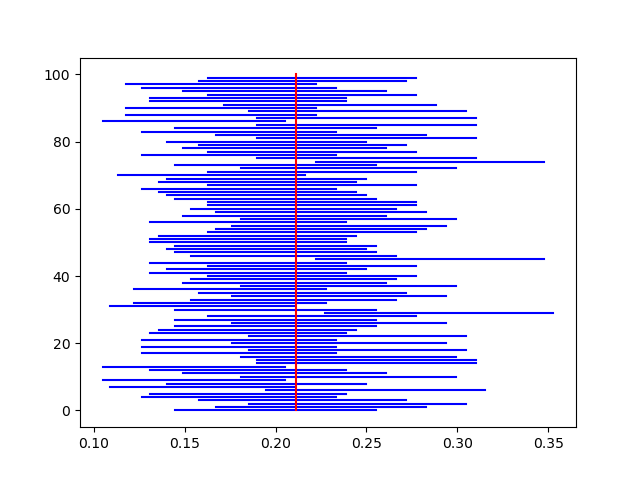
\includegraphics[scale=0.5]{1d.png}
            \label{slika 1d}
            \caption{Intervali zaupanja za $100$ enostavnih slučajnih vzorcev
            velikosti $200$. Z rdečo je označeno populacijsko povprečje.}
        \end{figure}
    \item Standardni odklon vzorčnih deležev je približno $0{,}02902$, kar je
        približno enako kot standardna napaka za vzorec velikosti $200$.
    \item Sedaj pa izvedimo podobno še na $100$ vzorcih velikosti $800$. Na
        sliki~\ref{slika 1f} vidimo, da so intervali v povprečju ožji kot na
        sliki~\ref{slika 1d}. To je zato, ker je standardni odklon vzorčnih
        deležev manjši, če vzamemo večje deleže. Standardni odklon vzorčnih
        deležev teh $100$ vzorcev velikosti $800$ je približno $0{,}01209$.
        Torej je res manjši od iste vrednosti za manjše vzorce. Prava standardna
        napaka za vzorec velikosti pa je enaka $0{,}01431$. Če bi vzeli več
        vzorcev, bi bil standardni odklon vzorčnih deležev v povprečju bližje
        pravi standardni napaki za vzorec te velikosti.
        \begin{figure}[H]
            \centering
            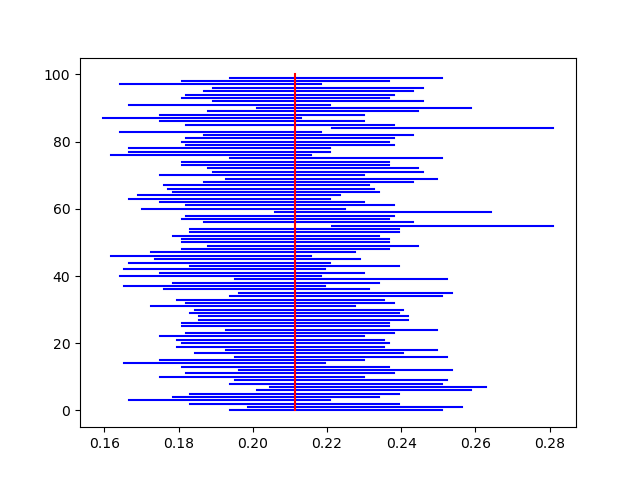
\includegraphics[scale=0.5]{1f.png}
            \label{slika 1f}
            \caption{Intervali zaupanja za $100$ enostavnih slučajnih vzorcev
            velikosti $800$. Z rdečo je označeno populacijsko povprečje.}
        \end{figure}
\end{enumerate}

\section{Druga naloga}

Pri drugi nalogi smo opazovali normalnost empirične porazdelitve. V obdobju $24$
dni so vsak dan analizirali pet odlitkov. Te odlitke sem združil v 
seznam dolžine $120$, ki vsebuje vrednosti vseh odvzetih odlitkov.

\begin{figure}[H]
    \centering
    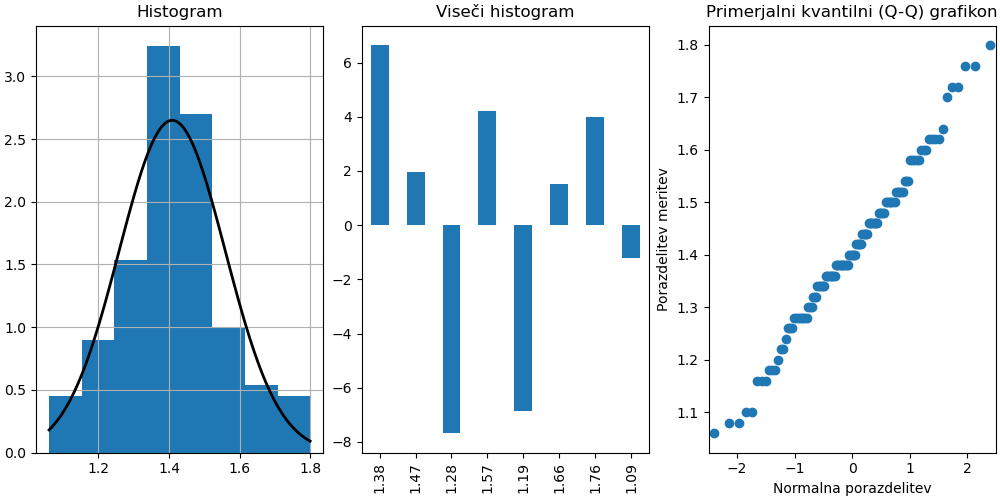
\includegraphics[scale=0.45]{2.png}
    \caption{Na levi strani je histogram, kjer so prikazani vsi odlitki, hkrati
    je pa dorisana krivulja normalne porazdelitve, ki to empirično porazdelitev
    najbolje aproksimira. Na sredini je viseči histogram, ki za vsak razred
    podatkov nariše razliko med pričakovanim deležem podatkov in empiričnem
    deležem podatkov v tem razredu. Na desni pa je primerjalni kvantilni (Q-Q)
    diagram, ki primerja normalno in empirično porazdelitev.}
    \label{slika 2}
\end{figure}

Podatke smo združili v razrede po modificiranem Freedman-Diaconisovem pravilu.
Najprej smo izračunali interkvartilni razmik po enačbi
\begin{equation*}
    IQR = x_\frac{3}{4} - x_\frac{1}{4},
\end{equation*}
kjer sta $x_\frac{3}{4}$ tretji kvartil in $x_\frac{1}{4}$ prvi kvartil. Nato
smo z uporabo interkvartilnega razmika izračunali še širino intervalov $d$ po
formuli
\begin{equation*}
    d = \frac{2{,}6\ IQR}{\sqrt[3]{n}}.
\end{equation*}
V našem primeru po tej metodi širina intervalov znaša $0{,}09488$.

\section{Tretja naloga}

Pri tretji nalogi obravnavamo mesečne temperature v Ljubljani v letih od 1986 do
2020. Najprej sem podatke združil v seznam dolžine $420$.

Obravnaval bom model A, ki je linearen trend s sinusnim nihanjem s periodo eno
leto, in model B, ki je linearen trend s spreminjanjem temperature vsak mesec
posebej. Model A lahko opišemo s konfiguracijsko matriko
\[
    X_A =
    \left[ {\begin{array}{cccc}
        1 & 0 & 0 & 1\\
        1 & 1 & \sin(\frac{\pi}{6}) & \cos(\frac{\pi}{6})\\
        1 & 2 & \sin(\frac{2 \pi}{6}) & \cos(\frac{2 \pi}{6})\\
        1 & 3 & \sin(\frac{3 \pi}{6}) & \cos(\frac{3 \pi}{6})\\
        \vdots & \vdots & \vdots & \vdots\\
        1 & 418 & \sin(\frac{418 \pi}{6}) & \cos(\frac{418 \pi}{6})\\
        1 & 419 & \sin(\frac{419 \pi}{6}) & \cos(\frac{419 \pi}{6})\\
    \end{array} } \right],
\]
model B pa z matriko
\[
    X_B =
    \left[ {\begin{array}{ccccccccccccc}
        0 & 1 & 0 & 0 & 0 & 0 & 0 & 0 & 0 & 0 & 0 & 0 & 0\\
        1 & 0 & 1 & 0 & 0 & 0 & 0 & 0 & 0 & 0 & 0 & 0 & 0\\
        2 & 0 & 0 & 1 & 0 & 0 & 0 & 0 & 0 & 0 & 0 & 0 & 0\\
        3 & 0 & 0 & 0 & 1 & 0 & 0 & 0 & 0 & 0 & 0 & 0 & 0\\
        4 & 0 & 0 & 0 & 0 & 1 & 0 & 0 & 0 & 0 & 0 & 0 & 0\\
        5 & 0 & 0 & 0 & 0 & 0 & 1 & 0 & 0 & 0 & 0 & 0 & 0\\
        6 & 0 & 0 & 0 & 0 & 0 & 0 & 1 & 0 & 0 & 0 & 0 & 0\\
        \vdots & \vdots & \vdots & \vdots & \vdots & \vdots & \vdots & \vdots &
        \vdots & \vdots & \vdots & \vdots & \vdots\\
        417 & 0 & 0 & 0 & 0 & 0 & 0 & 0 & 0 & 0 & 1 & 0 & 0\\
        418 & 0 & 0 & 0 & 0 & 0 & 0 & 0 & 0 & 0 & 0 & 1 & 0\\
        419 & 0 & 0 & 0 & 0 & 0 & 0 & 0 & 0 & 0 & 0 & 0 & 1\\
    \end{array} } \right].
\]

Na predavanjih smo pokazali, da je ocena za vektor $\beta$ po metodi največjega
verjetja enaka vektorju $\hat{\beta} = \left( X^\mathrm{T} X\right)^{-1}
X^\mathrm{T} Y$, kar je natanko rešitev predoločenega sistema $X \beta = Y$ po
metodi najmanjših kvadratov (s predpostavko, da je $X$ polnega ranga). Tu je $Y$
vektor opažanj.

Označimo z $\beta_A$ in $\beta_B$ oceni parametrov modelov A in B.
S programom \textbf{naloga3.py} izračunamo
\begin{equation*}
    \hat{\beta_A} = \left[ \begin{array}[c]
        & 0.001\\ 0.091\\ -10.39\\
    \end{array} \right]
    \quad \text{in} \quad
    \hat{\beta_B} = \left[ \begin{array}
        & 0.005\\ -11.504\\ -9.801\\ -5.486\\ -0.949\\ 3.617\\ 7.28\\ 9.292\\ 8.733\\
        3.704\\ -1.033\\ -6.301\\ -11.095\\
    \end{array} \right].
\end{equation*}
Rezultati se zdijo smiselni, saj bo nihanje skozi leto res izgledalo podobno
grafu nasprotne vrednosti kosinusa. Podobno iz $\hat{\beta_B}$ razberemo, da so
pozimi temperature nižje od povprečja, poleti pa višje. Prvi komponenti vektorjev
$\hat{\beta_A}$ in $\hat{\beta_B}$ predstavljata linearen trend, ki je pri obeh
modelih pozitiven, torej so se temperature v opazovanem času v povprečju
dvignile.


\begin{figure}[H]
    \centering{}
    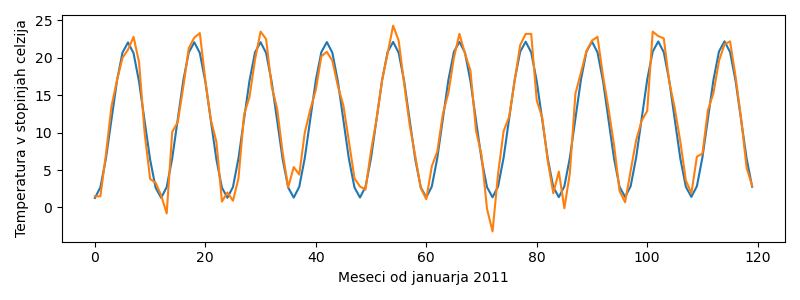
\includegraphics[scale=0.6]{3a.png}
    \caption{Na grafikonu sta narisani dve krivulji. Oranžna označuje empirične
    podatke, modra pa oceno znotraj modela A.}
    \label{slika 3a}
\end{figure}

\begin{figure}[H]
    \centering{}
    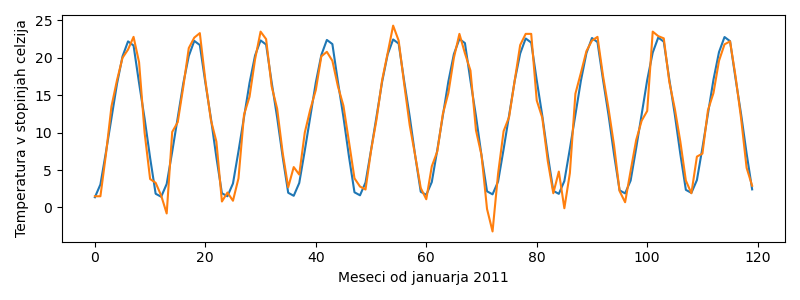
\includegraphics[scale=0.6]{3b.png}
    \caption{Na grafikonu sta narisani dve krivulji. Oranžna označuje empirične
    podatke, modra pa oceno znotraj modela B.}
    \label{slika 3b}
\end{figure}

Pri drugem delu naloge smo izračunali Akaikejevo informacijo 


% \nocite{*}
% \bibliographystyle{siam}
% \bibliography{viri}{}

\end{document}
